\subsection{Квадратная волна}

Рассмотрим периодическую функцию с периодом $T = 3$:
\begin{equation}
    f_1(t) = 
    \begin{cases}
        1, & t \in [1, 2) \\
        2, & t \in [2, 4)
    \end{cases}
    \label{eq:func_1}
\end{equation}

График этой функции приведен на рис.~\ref{fig:func_1}. 
\begin{figure}[ht!]
    \centering
    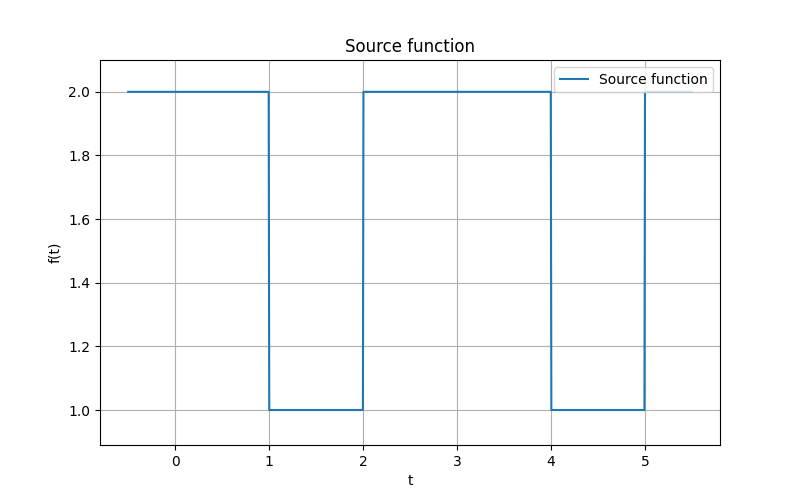
\includegraphics[width=\textwidth]{media/plots/func_1.png}
    \caption{График функции $f_1(t)$}
    \label{fig:func_1}
\end{figure}

\subsubsection{Вычисление коэффициентов Фурье}
Найдем частичные суммы ряда Фурье для этой функции:

Вычислим коэффициенты $a_n$, $b_n$ и $c_n$ для $n = 0, 1, 2$ в соответствии с формулами (\ref{eq:fourier_coefficients}) и (\ref{eq:fourier_coefficients_exp}): 

\begin{equation}
    a_n = \frac{2}{3} \int\limits_{1}^{4} f_1(t) \cos\left( \frac{2\pi n}{3} t\right) dt = \frac{2}{3} \left( \int\limits_{1}^{2} \cos\left( \frac{2\pi n}{3} t\right) dt + \int\limits_{2}^{4} 2 \cos\left( \frac{2\pi n}{3} t\right) dt \right) 
\end{equation}
\begin{equation}
    \int \cos\left( \frac{2\pi n}{3} t \right) dt = \int \frac{3\cos(u)}{2\pi n}du = \frac{3}{2\pi n } \sin(u) = \frac{3}{2\pi n } \sin\left( \frac{2\pi n}{3} t \right)
    \notag
 \end{equation}
\begin{multline}
    a_n = \frac{2}{3} \left( \frac{3}{2\pi n } \sin\left( \frac{2\pi n}{3} t \right) \Big|_{1}^{2}  + \frac{3}{\pi n } \sin\left( \frac{2\pi n}{3} t \right) \Big|_2^4 \right) = \\ 
    \frac{2}{\pi n} \left( \frac{1}{2} \left( \sin\left(\frac{4\pi n}{3}\right) - \sin\left(\frac{2\pi n}{3}\right) \right) + \left(\sin\left(\frac{8\pi n}{3}\right)  - \sin\left(\frac{4\pi n}{3}\right)  \right) \right) = \\
    \frac{1}{\pi n}\left(-\sin\left( \frac{4\pi n}{3}\right) - \sin\left(\frac{2\pi n}{3} \right) + 2\sin\left(\frac{8\pi n}{3}\right)\right)
\end{multline}
\begin{equation}
    b_n = \frac{2}{3} \int\limits_{1}^{4} f_1(t) \sin\left( \frac{2\pi n}{3} t\right) dt = \frac{2}{3} \left( \int\limits_{1}^{2} \sin\left( \frac{2\pi n}{3} t\right) dt + \int\limits_{2}^{4} 2 \sin\left( \frac{2\pi n}{3} t\right) dt \right) 
\end{equation}
\begin{equation}
    \int \sin\left( \frac{2\pi n}{3} t \right) dt = \int \frac{3\sin(u)}{2\pi n}du = \frac{-3}{2\pi n } \cos(u) = \frac{-3}{2\pi n } \cos\left( \frac{2\pi n}{3} t \right)
    \notag
 \end{equation}
\begin{multline}
    b_n = \frac{2}{3} \left( \frac{-3}{2\pi n } \cos\left( \frac{2\pi n}{3} t \right) \Big|_{1}^{2}  + \frac{-3}{\pi n } \cos\left( \frac{2\pi n}{3} t \right) \Big|_2^4 \right) = \\ 
    \frac{-2}{\pi n} \left( \frac{1}{2} \left( \cos\left(\frac{4\pi n}{3}\right) - \cos\left(\frac{2\pi n}{3}\right) \right) + \left(\cos\left(\frac{8\pi n}{3}\right)  - \cos\left(\frac{4\pi n}{3}\right)  \right) \right) = \\
    \frac{1}{\pi n}\left(\cos\left( \frac{4\pi n}{3}\right) + \cos\left(\frac{2\pi n}{3} \right) - 2\cos\left(\frac{8\pi n}{3}\right)\right)
\end{multline}
\begin{equation}
    c_n = \frac{1}{3}\int\limits_{1}^{4} f_1(t)e^{\frac{-i 2\pi n t}{3}} dt = \frac{1}{3}\left(\int\limits_{1}^{2}e^{\frac{-i 2\pi n t}{3}}dt + \int\limits_{2}^{4}2e^{\frac{-i 2\pi n t}{3}}dt \right) 
\end{equation}
Так как коэффициенты $a_n$, $b_n$ и $c_n$ связаны между собой, а $c_i$ и $c_{-i}$ равны для вещественной функции, нет необходимости вычислять $c_n$ отдельно. (Мне просто лень). 
\begin{equation}
    c_n = \frac{a_n - ib_n}{2}
\end{equation}
После подстановки получаем следующие значения:
\begin{equation}
    a_0 = \frac{2}{3} \int\limits_{1}^{4} f_1(t) dt = \frac{2}{3} \left( \int\limits_{1}^{2} dt + \int\limits_{2}^{4} 2 dt \right) = \frac{2}{3} \left(t\Big|_{1}^{2} + 2t\Big|_{2}^{4}\right) = \frac{2}{3} (1 + 4) = \frac{10}{3} \approx 3.33333
\end{equation}

\begin{equation}
    a_1 = \frac{1}{\pi}\left(-\sin\left( \frac{4\pi}{3}\right) - \sin\left(\frac{2\pi}{3} \right) + 2\sin\left(\frac{8\pi}{3}\right)\right) = \frac{\sqrt3}{3} \approx 0.55133 
\end{equation}

\begin{equation}
    a_2 = \frac{1}{2\pi}\left(-\sin\left( \frac{8\pi}{3}\right) - \sin\left(\frac{4\pi}{3} \right) + 2\sin\left(\frac{16\pi}{3}\right)\right) = \frac{-\sqrt{3}}{2\pi} \approx -0.27567
\end{equation}

\begin{equation}
    b_1 = \frac{1}{\pi}\left(\cos\left( \frac{4\pi}{3}\right) + \cos\left(\frac{2\pi}{3} \right) - 2\cos\left(\frac{8\pi}{3}\right)\right) = 0
\end{equation}

\begin{equation}
    b_2 = \frac{1}{2\pi}\left(\cos\left( \frac{8\pi}{3}\right) + \cos\left(\frac{4\pi}{3} \right) - 2\cos\left(\frac{16\pi}{3}\right)\right) = 0
\end{equation}

\begin{equation}
    c_0 = \frac{a_0}{2} = \frac{10}{6} \approx 1.66667
\end{equation}

\begin{equation}
    c_{-1} = c_1 = \frac{a_1 - b_1}{2} = \frac{\sqrt3}{6} \approx 0.28868
\end{equation}

\begin{equation}
    c_{-2} = c_2 = \frac{a_2 - b_2}{2} = \frac{-\sqrt{3}}{4\pi} \approx -0.13784
\end{equation}

\subsubsection{Вычисление коэффициентов Фурье с помощью программы}
Воспользуемся программой для вычисления коэффициентов Фурье. Исходный код всех функций приведен в дополнении \ref{appendix:source}.

\begin{lstlisting}[style=python_white, caption=Вычисление коэффициентов Фурье, label=lst:func_1]
func = np.vectorize(lambda x: 1 if 0 <= (x - 1) % 3 < 1 else 2)
a, b = fourier(func, 0, 2 * np.pi, 3)
print_fourier_coefficients(a, b)
c = fourier_exp(func, 1, 3, 3)
print_fourier_exp_coefficients(c)
\end{lstlisting}

В результате выполнения программы (\ref{lst:func_1}) получим следующие значения (см. таблицу~\ref{tab:func_1}~и~\ref{tab:func_1_exp}).

% table with coefficients
\begin{table}[ht!]
    \centering
    \begin{tabular}{|c|c|c|c|}
        \hline
        $n$ & $a_n$ & $b_n$ \\
        \hline
        0 & 3.33335 & 0.0 \\
        1 & 0.55123 & 0.0 \\
        2 & -0.2757 & 0.0 \\
        3 & 0.00020 & 0.0 \\
        \hline
    \end{tabular}
    \caption{Коэффициенты Фурье для функции $f_1(t)$}
    \label{tab:func_1}
\end{table}

\begin{table}[ht!]
    \centering
    \begin{tabular}{|c|c|}
        \hline
        $n$ & $c_n$ \\
        \hline
        -3 & 0.00010 \\
        -2 & -0.13788 \\
        -1 & 0.27561 \\
        0 & 1.66677 \\
        1 & 0.27561 \\
        2 & -0.13788 \\
        3 & 0.00010 \\
        \hline
    \end{tabular}
    \caption{Коэффициенты Фурье для функции $f_1(t)$ (комплексный случай)}
    \label{tab:func_1_exp}
\end{table}

Полученные коэффициенты совпадают с вычисленными вручную значениями.

\subsubsection{Построение графиков частичных сумм ряда Фурье}
В качество значений $N$ выберем $N = 1, 2, 5, 15, 30$. Для каждого значения $N$ вычислим частичную сумму ряда Фурье и построим график (см. рис.~\ref{fig:func_1_plot}~и~\ref{fig:func_1_plot_exp}).

\begin{lstlisting}[style=python_white, caption=Построение графиков частичных сумм ряда Фурье, label=lst:func_1_plot]
func = np.vectorize(lambda x: 1 if 0 <= (x - 1) % 3 < 1 else 2)
calc_and_plot(func, 1, 3, [1, 2, 5, 15, 30], './media/plots/func_1')
calc_and_plot_exp(func, 1, 3, [1, 2, 5, 15, 30], './media/plots/func_1_exp')
\end{lstlisting}

% plot with partial sums
\begin{figure}[ht!]
    \centering
    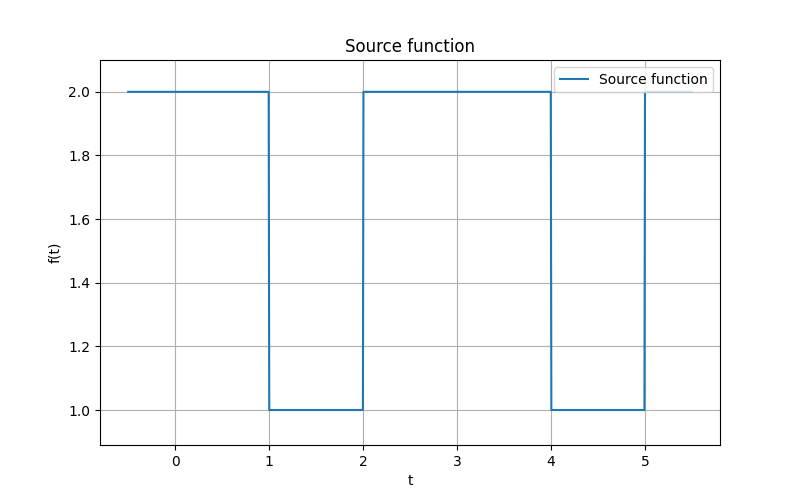
\includegraphics[width=0.49\textwidth]{media/plots/func_1.png}
    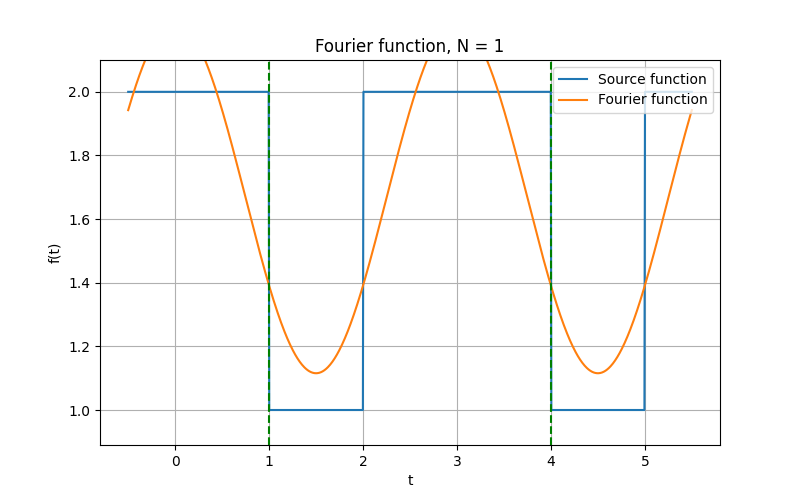
\includegraphics[width=0.49\textwidth]{media/plots/func_1_N_1.png}
    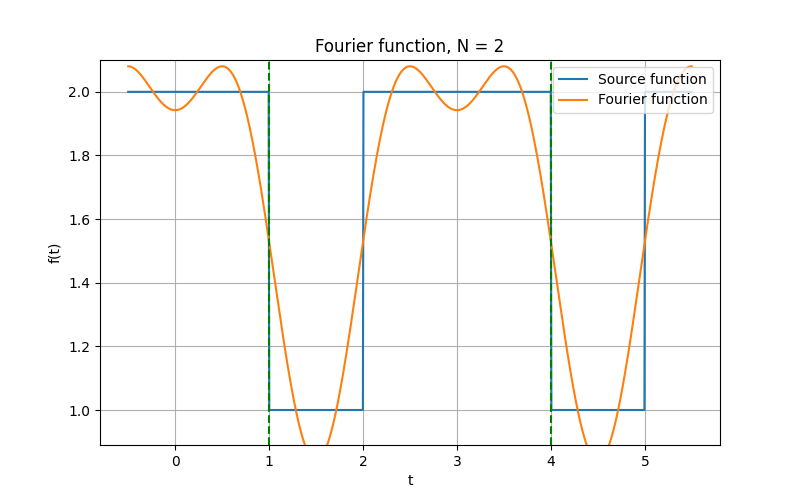
\includegraphics[width=0.49\textwidth]{media/plots/func_1_N_2.png}
    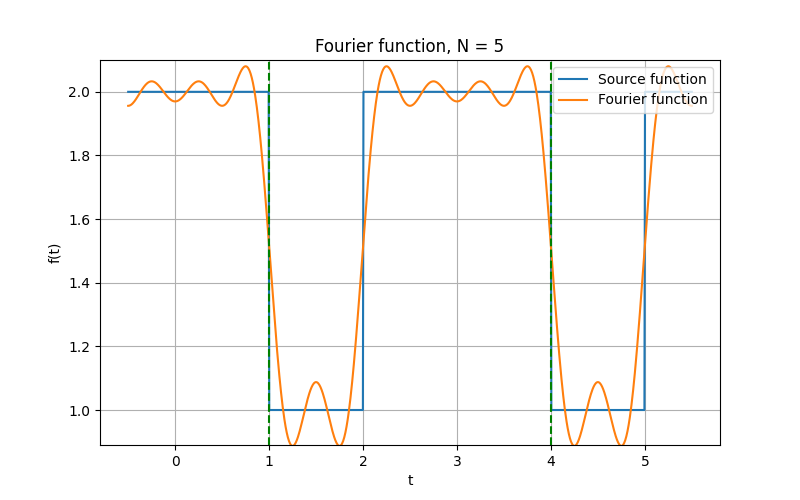
\includegraphics[width=0.49\textwidth]{media/plots/func_1_N_5.png}
    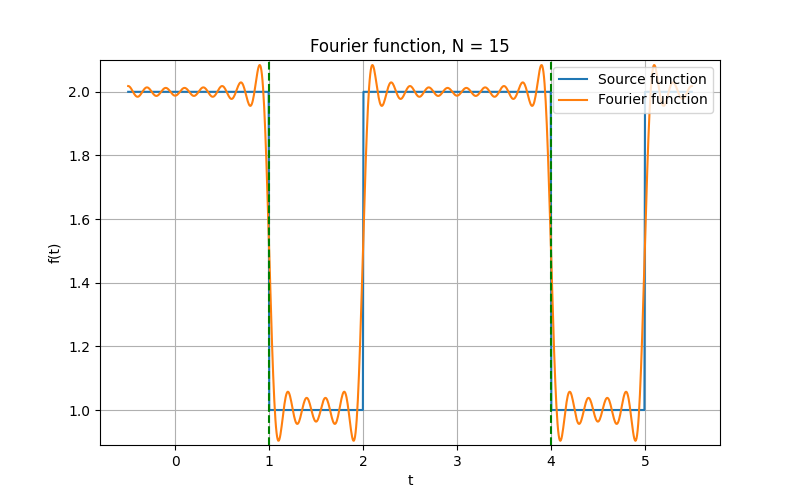
\includegraphics[width=0.49\textwidth]{media/plots/func_1_N_15.png}
    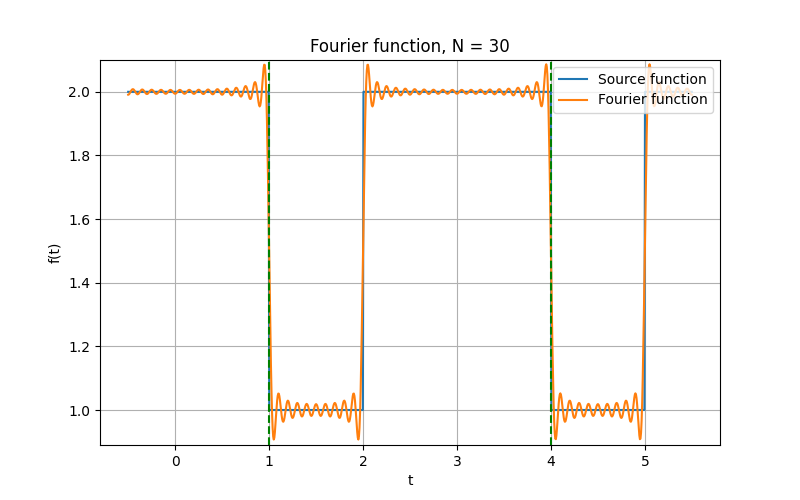
\includegraphics[width=0.49\textwidth]{media/plots/func_1_N_30.png}
    \caption{График частичных сумм ряда Фурье для функции $f_1(t)$}
    \label{fig:func_1_plot}
\end{figure}

\begin{figure}[ht!]
    \centering
    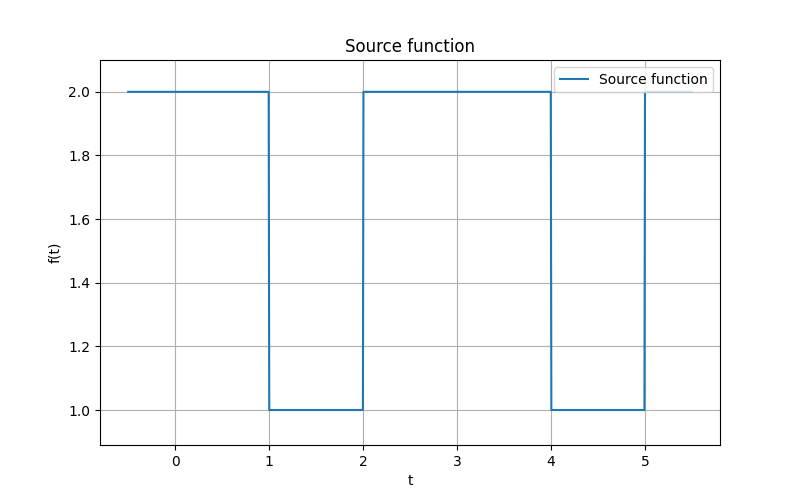
\includegraphics[width=0.49\textwidth]{media/plots/func_1_exp.png}
    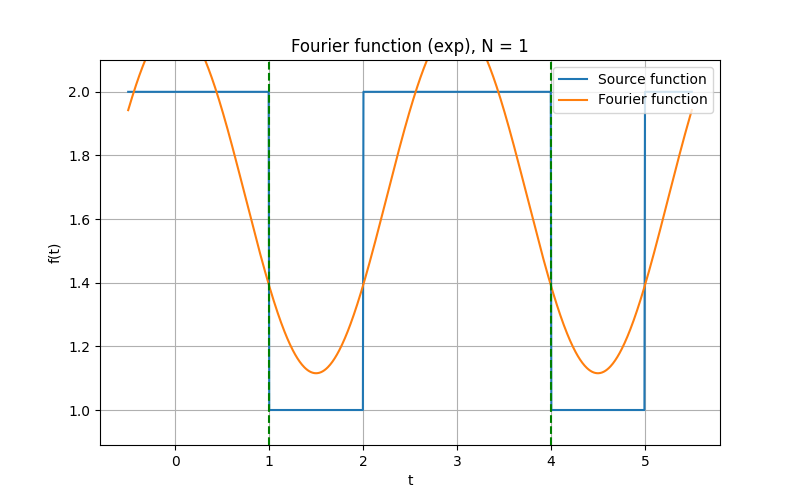
\includegraphics[width=0.49\textwidth]{media/plots/func_1_exp_N_1.png}
    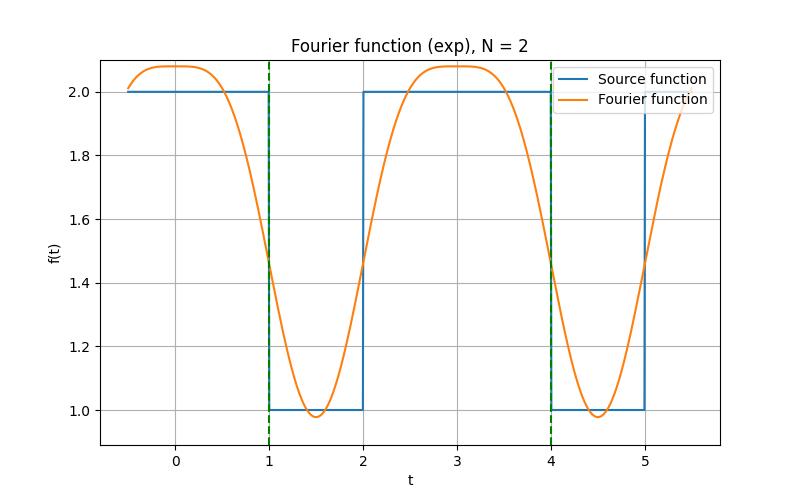
\includegraphics[width=0.49\textwidth]{media/plots/func_1_exp_N_2.png}
    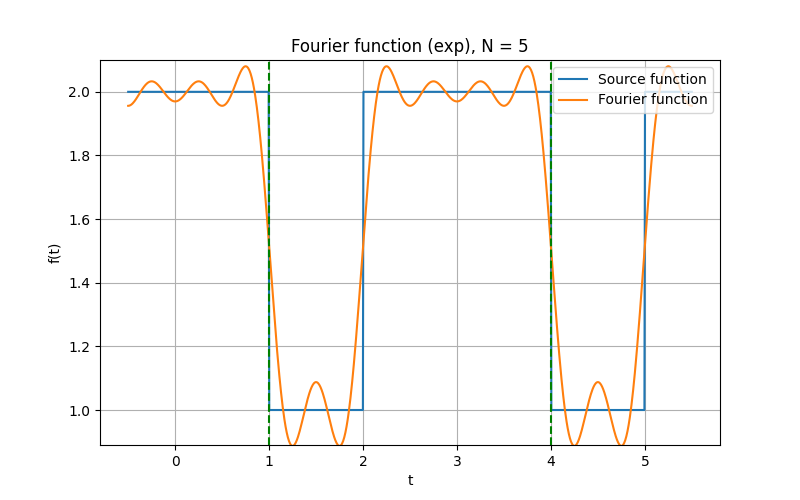
\includegraphics[width=0.49\textwidth]{media/plots/func_1_exp_N_5.png}
    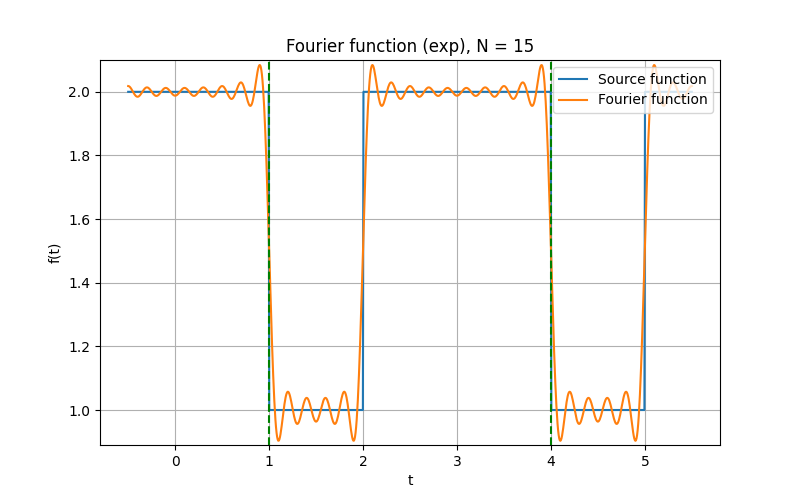
\includegraphics[width=0.49\textwidth]{media/plots/func_1_exp_N_15.png}
    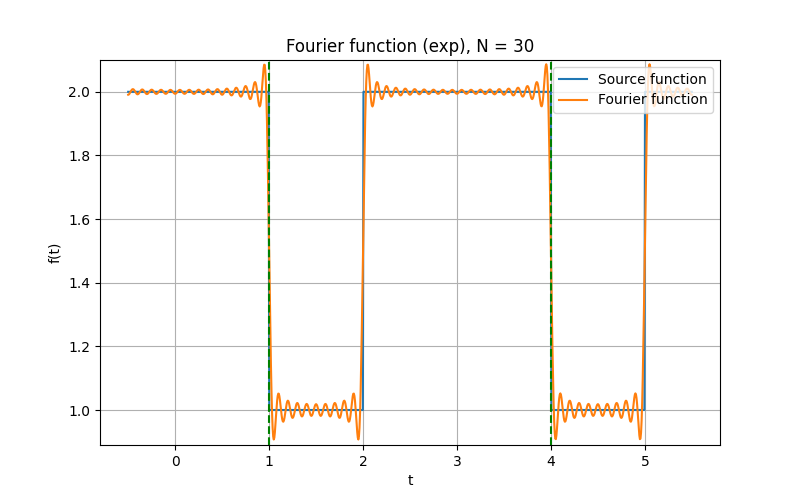
\includegraphics[width=0.49\textwidth]{media/plots/func_1_exp_N_30.png}
    \caption{График частичных сумм ряда Фурье для функции $f_1(t)$ (комплексный случай)}
    \label{fig:func_1_plot_exp}
\end{figure}

Видим, что при увеличении $N$ график частичной суммы ряда Фурье приближается к исходной функции. При $N = 5$ график частичной суммы ряда Фурье уже довольно хорошо приближает исходную функцию. 

На графиках заметны \textit{выбросы} в точках разрыва. Это связано с тем, что ряд Фурье сходится к функции по норме, но не обязательно в каждой точке. 

\FloatBarrier
\subsubsection{Проверка равенства Парсеваля}

Проверим равенство Парсеваля для функции $f_1(t)$:

\begin{equation}
    ||f_1||^2 = 2\pi \sum\limits_{n = -\infty}^{\infty} |c_n|^2 
\end{equation}

\begin{equation}
    ||f_1||^2 = \pi \left(\frac{a_0^2}{2} + \sum\limits_{n = 0}^{\infty}  (a_n^2 + b_n^2) \right)
\end{equation}

Для этого воспользуемся функцией \texttt{perseval\_check} (см. листинг~\ref{lst:perseval_check}).
Мною была рассмотрена сумма трехсот коэффициентов. Этого оказалось достаточно для равенства квадрата нормы и суммы до 3 знака. 

\begin{table}[ht!]
    \centering
    \begin{tabular}{|c|c|c|}
        \hline
        $||f_1||^2$ & $2\pi \sum\limits_{n = -\infty}^{300} |c_n|^2$ & $\pi \left(\frac{a_0^2}{2} + \sum\limits_{n = 1}^{300} (a_n^2 + b_n^2)\right)$\\
        \hline
        19.13296 & 19.13141 & 19.13141\\
        \hline
    \end{tabular}
    \caption{Проверка равенства Персеваля для функции $f_1(t)$}
    \label{tab:func_1_pers}
\end{table}
